\documentclass{article}
\usepackage[12pt]{extsizes}
\usepackage[T2A]{fontenc}
\usepackage[utf8]{inputenc}
\usepackage[english, russian]{babel}

\usepackage{amssymb}
\usepackage{amsfonts}
\usepackage{amsmath}
\usepackage{enumitem}
\usepackage{graphics}
\usepackage{graphicx}

\usepackage{lipsum}
\DeclareGraphicsExtensions{.pdf,.png,.jpg}



\usepackage{geometry} % Меняем поля страницы
\geometry{left=1cm}% левое поле
\geometry{right=1cm}% правое поле
\geometry{top=1.5cm}% верхнее поле
\geometry{bottom=1cm}% нижнее поле


\usepackage{fancyhdr} % Headers and footers
\pagestyle{fancy} % All pages have headers and footers
\fancyhead{} % Blank out the default header
\fancyfoot{} % Blank out the default footer
\fancyhead[L]{ЦРОД $\bullet$ Математика}
\fancyhead[C]{\textit{Немного алгебры}}
\fancyhead[R]{Стратегия 2021}% Custom header text


%----------------------------------------------------------------------------------------

%\begin{document}\normalsize
\begin{document}\large
	

\begin{center}
\textbf{Многочлены}
\end{center}

\begin{enumerate}[label*=\protect\fbox{\arabic{enumi}}]

\item Решите уравнение:  $x(x + 1) = 2020\cdot2021$

\item При каких $p$ и $q$ уравнению  $x^2 + px + q = 0$  удовлетворяют два различных числа $2p$ и  $p + q$?

\item Пусть $x_1, x_2$~--- корни уравнения  $x^2 + px + q = 0$.  Выразите через $p$ и $q$ следующие выражения: 
\begin{enumerate}
	
	\item $\dfrac{1}{x_1} + \dfrac{1}{x_2}$
	
	\item $\dfrac{1}{x_1^2} + \dfrac{1}{x_2^2}$
	
\end{enumerate}

\item Рассматриваются квадратичные функции  $y = x^2 + px + q$,  для которых  $p + q = 2021$.
Покажите, что параболы, являющиеся графиками этих функций, пересекаются в одной точке.

\item Существуют ли такие три квадратных трёхчлена, что каждый из них имеет корень, а сумма любых двух из них корней не имеет?

\item Два различных числа $x$ и $y$ (не обязательно целых) таковы, что $$x^2 - 2000x = y^2 - 2000y$$.  Найдите сумму чисел $x$ и $y$.

\item Квадратный трехчлен  $y = ax^2 + bx + c$  не имеет корней и  $a  + b + c > 0$.  Найдите знак коэффициента $с$.

\item Верно ли, что если  $b > a + c > 0$,  то квадратное уравнение $ax^2 + bx + c = 0$ имеет два корня?

\item Найдите сумму всех коэффициентов многочлена  $(3x^2 - 4x + 2)^{2021}$ после раскрытия скобок и приведения подобных членов.

\item Докажите, что если в выражении  $(x^2 - x + 1)^{2021}$  раскрыть скобки и привести подобные слагаемые, то какой-нибудь коэффициент полученного многочлена будет отрицательным.

\item Про действительные числа $a, b, c$ известно, что $(a + b + c)\cdot c < 0$. Докажите, что $b^2 - 4ac>0$.

\newpage
\item Докажите теорему Виета для кубического многочлена:

\textbf{Теорема Виета для кубического многочлена} 

Если кубическое уравнение $ax^3 + bx^2 + cx + d = 0$ имеет три корня $x_1, x_2, x_3$, то $$x_1 + x_2 + x_3 = -\dfrac{b}{a}$$ $$x_1x_2  + x_2x_3 + x_1x_3 = \dfrac{c}{a}$$ $$x_1x_2x_3 = -\dfrac{d}{a}$$

\item Известно, что уравнение  $x^3 + ax + b = 0$  имеет три решения $x_1, x_2, x_3$, и $x_1 = -x_3$. Чему равен коэффициент $b$?

\item Прямые, параллельные оси $Ox$, пересекают график функции  $y = ax^3 + bx^2 + cx + d$:  первая – в точках $A, D$ и $E$, вторая – в точках $B, C$ и $F$ (см. рис.). Докажите, что длина проекции дуги $CD$ на ось $Ox$ равна сумме длин проекций дуг $AB$ и $EF$.
\begin{figure}[h]
	\center{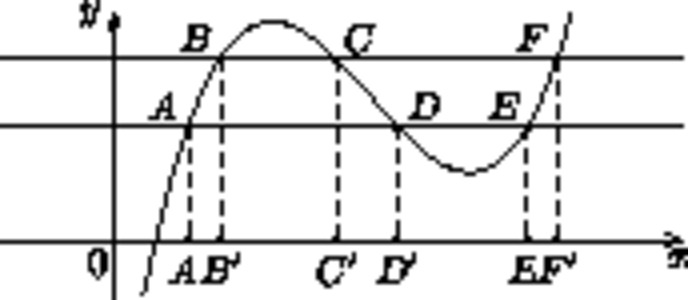
\includegraphics[scale=0.5]{document}}
	\label{fig:image}
\end{figure}

\item \textbf{Теорема Безу}: Пусть $P(x)$~--- многочлен с целыми коэффициентами, $a$ и $b$~--- различные целые числа. Тогда $P (a) - P (b)$ делится на $a - b$.

\item Докажите, что не существует многочлена $P(x)$ с целыми коэффициентами, для которого $P(6) = 5$ и $P(14) = 9$.

\item Докажите, что многочлен $P(x) = (x + 1)^6 - x^6- 2x - 1$ делится на $x(x+1)(2x+1)$.

\item Какой остаток даёт $x+x^{3} +x^{9} +x^{27} +x^{81} +x^{243}$ при делении на $x-1$?

\item Докажите, что любой многочлен нечётной степени имеет хотя бы один корень


\end{enumerate}
\end{document}